\section{Исследование прототипа детектора для установки <<Лазерный поляриметр>>}
\label{sec:pol_examine}
\subsection{Конструкция детектора}
Для регистрации одиночных гамма--квантов, полученных обратным комптоновским рассеянием на пучках электронов, был спроектирован и изготовлен прототип детектора, использующего ГЭУ для усиления сигнала первичной ионизации. В конструкции применен тройной электрод с питанием от резистивного делителя. Основа детектора представляет собой многослойную плату из СТЭФ с массивом плоских металлических электродов, расположенных в её центральной части, которую можно видеть на Рис. \ref{fig:Pol_det_photo} 
\par Электроды поделены на группы, каждая из которых регистрируется отдельной считывающей платой. Всего считывающих плат десять, и они установлены в специальные многоканальные разъемы на периферии основной платы. Front-end электроника включает в себя быстрые АЦП и ПЛИС для работы с ними. Далее сигнал по USB подается на компьютер. На данный момент разрабатывается программное обеспечивающее взаимодействие всех 10 плат и одновременное считывание события с детектора. Решено было использовать для последующих экспериментов только одну из плат, т.к. вычитывание данных с неё уже отлажено. 
\par Электроды ГЭУ укреплены на рамках из 1.5 мм СТЭФ над считывающей структурой. Сверху на плату закрепляется герметичный кожух из СТЭФ с трубками для ввода и вывода газовой смеси. Сборка детектора осуществляется в корпусе из листового алюминия.
\par Данный детектор отличается от аналогов большей гранулярностью, что даст большую точность определения координат событий. (может ещё что написать)
\subsection{Особенности сбора и обработки сырых данных}
Каналы детектора объединены в группы по 100 (центральная часть) или 120 (периферия) каналов. Каждая группа скоммутирована на отдельный разъем, к которому подключены два многоканальных АЦП. Одновременно можно вычитывать данные со всех каналов. При поступлении сигнала с триггера, схема начинает последовательно раз в 125 нс вычитывать заряд со всех каналов. Таким образом вычитывание происходит 100 раз. Каждый отсчет времени будем в дальнейшем называть <<кадром>>, а массив данных о заряде для каждого из каналов группы и каждого кадра из 100 назовем <<событием>>. 
\par Из-за технических особенностей схемы нулевой уровень сигнала составляет 7400 каналов АЦП. Сигнал, соответствующий пришедшей на электрод ионизации, представляет собой импульс отрицательной полярности, который имеет резкий передний фронт (1 кадр) и экспоненциально затухающий задний фронт (3-10 кадров в зависимости от суммарного заряда). Для последующей обработки сигнала, из него необходимо вычесть пьедестал. С этой целью в программе управления считывающей платой реализована возможность получения усредненных данных о пьедесталах, которые затем записываются в отдельный файл формата TXT. На Рис. \ref{pedestal_map} представлены гистограммы для пьедесталов одной считывающей платы.
\begin{figure}[H]
\begin{center}
	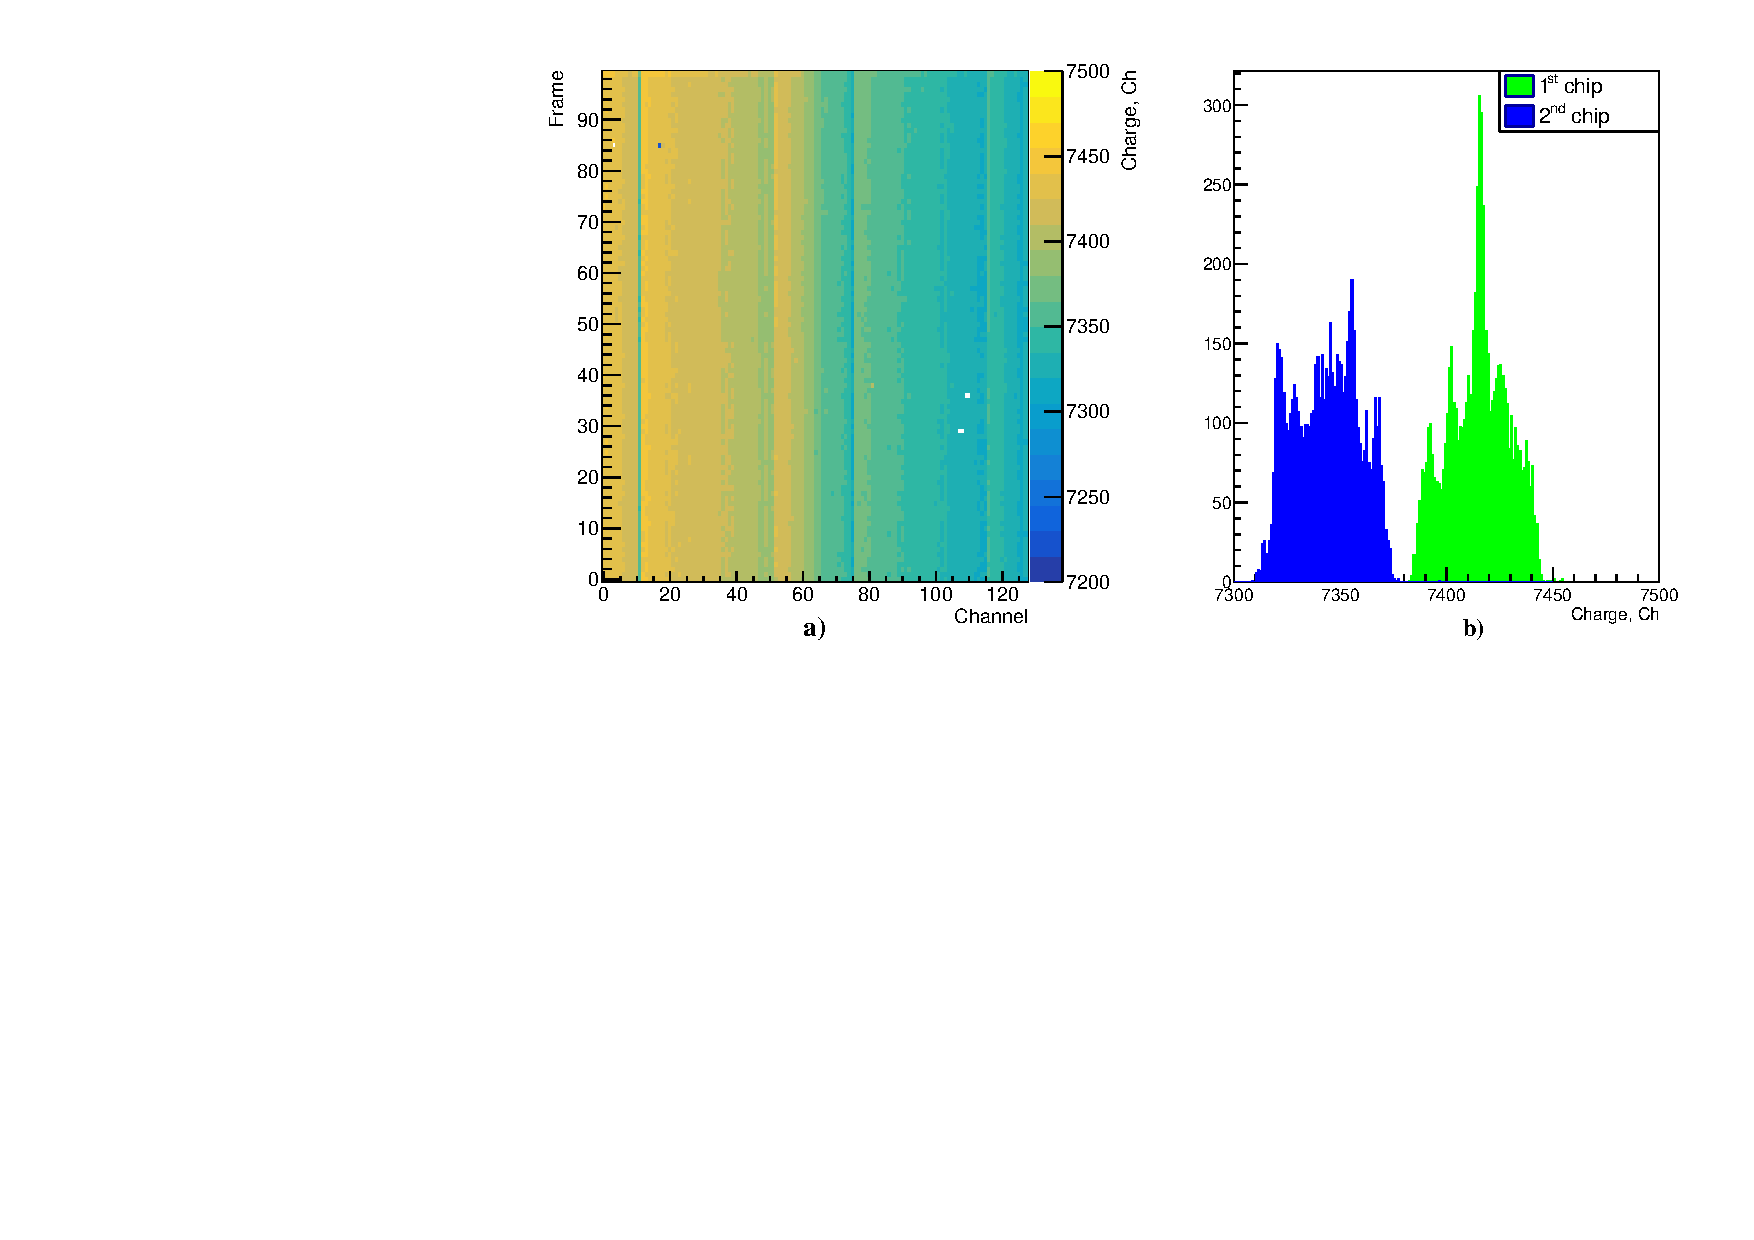
\includegraphics[width = 12cm]{img/pedestal_map.pdf}
	\caption{a): Карта пьедесталов АЦП. По горизонтальной оси обозначены номера каналов одной группы (Channel). По вертикальной оси --- кадры (Frame). Значения заряда показаны на цветовой шкале и лежат в пределах 7200--7500 каналов АЦП (Ch). b): Распределение заряда по каналам для первого и второго чипа считывающей платы}
	\label{pedestal_map}
\end{center}
\end{figure}
Можно заметить, что существует как разброс значений пьедестала в одном чипе, так и между чипами в плате. Поэтому решено было вычитать из сигнала пьедестал, соответствующий данному каналу.
\par События последовательно записываются в TXT---файл. Формат вывода следующий: строка соответствует одному кадру и состоит из 128 чисел. Всего таких строк в событии 100. 101--я строка содержит номер кадра, с которого началось вычитывание значений АЦП. Данная информация важна по следующей причине: микросхемы АЦП непрерывно вычитывают заряд с каналов, но ПЛИС возвращает событие только при активации триггера. Это сделано для того, чтобы исключить накопление заряда на входах АЦП и искажения данных о сигнале. Ввиду возможного разброса параметров электронных компонентов внутреннего pipeline АЦП, необходимо определять пьедесталы не только для каждого канала, но и для каждого кадра в канале. Поэтому номер канала в последней строке события дает необходимую привязку к физическим кадрам АЦП и позволяет правильно вычитать пьедесталы.
\par В ходе работы с прототипом детектора было обнаружено, что некоторые каналы имеют на порядок больший уровень шума, поэтому решено было их значения занулять и в анализе не использовать. 
\begin{figure}[H]
	\begin{center}
		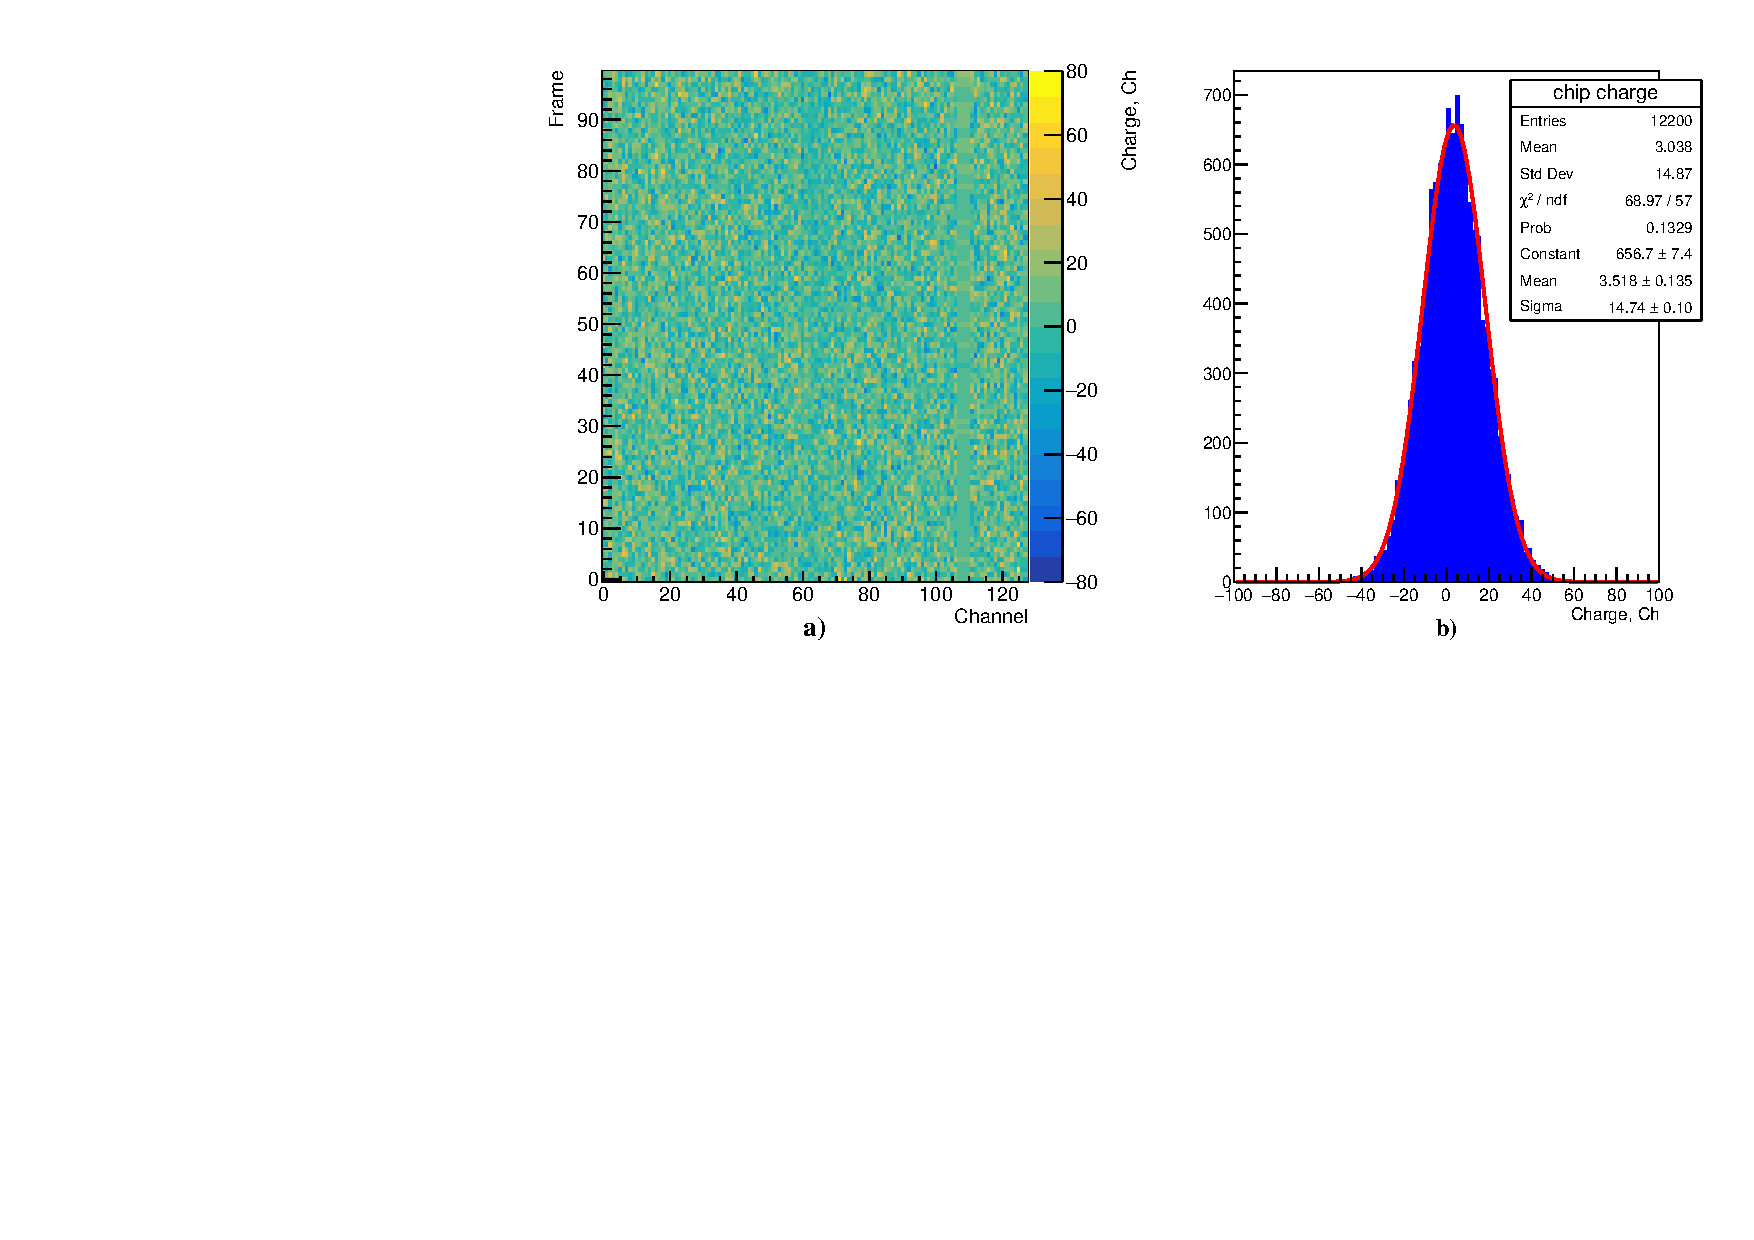
\includegraphics[width = 12cm]{img/noise_map.pdf}
		\caption{a): Вид шумового события после вычитания пьедестала b): Распределение заряда в шумовом событии}
		\label{noise_map}
	\end{center}
\end{figure}
Рис. \ref{noise_map} показывает вид одного шумового события и распределение заряда в кадрах и каналах. Важным значением, которое можно извлечь уже из одного шумового события является уровень шумов. Его можно определить как корень из дисперсии распределения на Рис. \ref{noise_map} b). Шумы в данном эксперименте составили $\approx15$ каналов АЦП. Если взять все шумовые события из файла сырых данных для конкретного эксперимента, то можно уточнить это значение, хотя, как показала практика, полученное по одному событию значение уже является достаточно хорошим приближением (тут нужно аргументировать!).
\subsection{Обработка сигнальных событий}
Сигнал, пришедший на электроды обычно распределяется по нескольким из них. Поэтому на мониторе события, который представлен на Рис. 
\begin{figure}[H]
	\begin{center}
		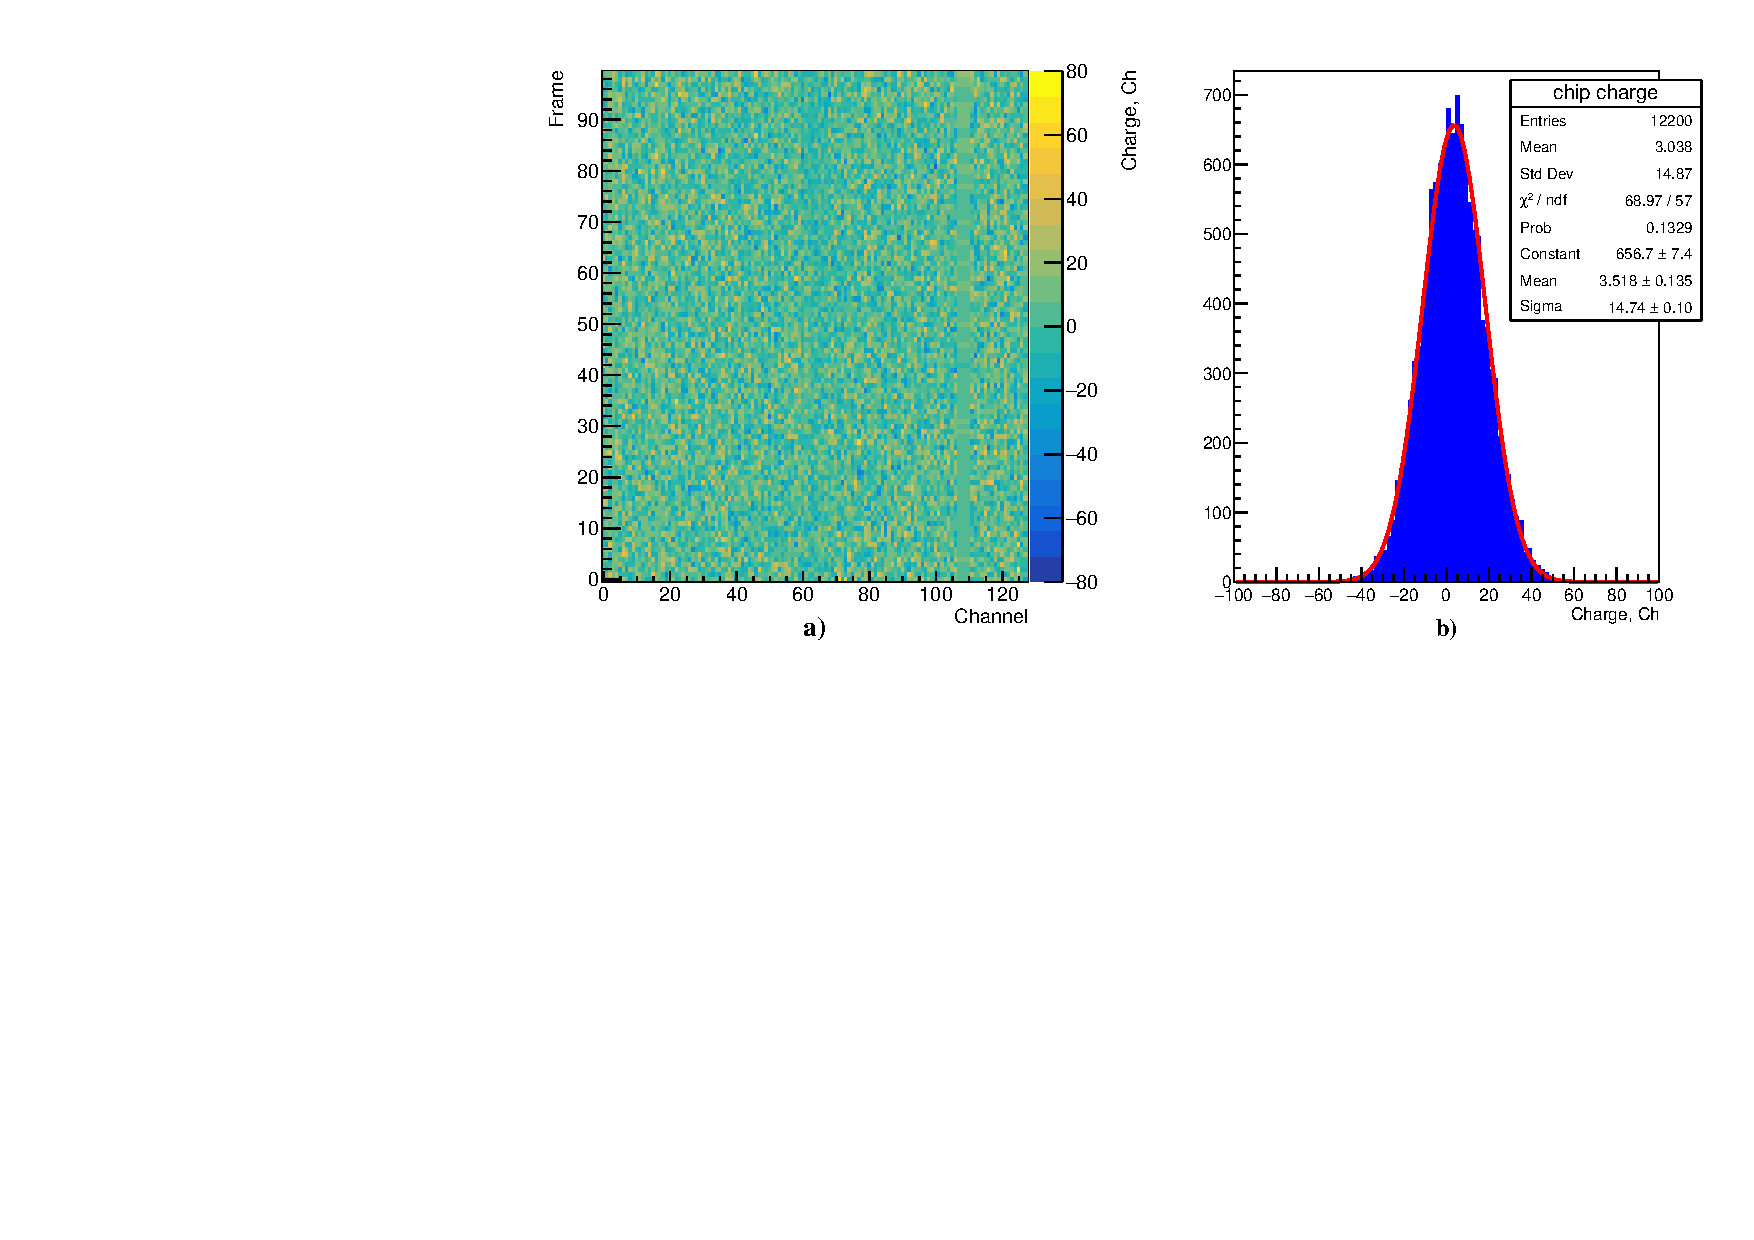
\includegraphics[width = 12cm]{img/noise_map.pdf}
		\caption{a): Вид шумового события после вычитания пьедестала b): Распределение заряда в шумовом событии}
		\label{event_map}
	\end{center}
\end{figure}
\subsection{Определение заряда кластера}
При приходе на считывающую структуру ионизации, заряд распределяется по электродам. Из-за этого обычно срабатывает не один канал, а целый кластер. 


Видно, что после вычитания пьедестала среднее значение шумов близко к нулю, но всё же не равно 
